\chapter{Metoder}\label{ch:met}
I dette kapitel vil vi redegøre for hvilke UX metoder vi har valgt at bruge i vores evaluering af Codecademy. Vi har valgt at begge metoder skal være meget forskellige fra hinanden, så de kan give os forskellige perspektiver. Begge er fundet igennem \textit{All About UX}\cite{AllAboutUX}.

\section{Affect Grid}\label{sec:AG}
Vi vil gerne vide, hvordan testpersoners oplevelse ændrer sig under interaktion med Codecademy. Vi har altså brug for en metode, der kan anvendes til at indsamle data flere gange under vores evaluering. 

Under evaluering kan det dog være svært, løbende at sætte sig ind i hvordan en testperson føler. Hvis evaluatoren hele tiden stiller dybdegående spørgsmål under evalueringen, risikerer vi at testpersonen bliver trukket ud af interaktionen. Dette kommer til at have indflydelse på personens oplevelse af produktet. Det vil altså være bedst hvis testpersonen selv kunne angive, hvordan de føler under evalueringen. Helst uden at de skal tænke for meget over det. 

Metoden vi vælger at anvende hedder \textit{Affect Grid}. Den er udviklet inden for psykologien af James A. Russel samt Anna Weiss og Gerald A. Mendelsohn \cite{AffectGrid}. Her angiver testpersonen selv deres følelsesmæssige tilstand, også kendt som \textit{affect}, på et såkaldt affect grid. Et blankt affect grid kan ses på \cref{fig:affectgrid}. Grid'et har en størrelse på 9*9 felter, X-aksen angiver fornøjelse(pleasure) og Y-aksen angiver ophidselse(arousal). Et 1 på X-aksen betyder stærk misfornøjelse, mens et 9 betyder stærk fornøjelse. Ligeledes betyder 1 på Y-aksen stærk søvnighed og 9 betyder stærk ophidselse. Hele metoden baserer sig på, at fornøjelse og ophidselse er uafhængige af hinanden. 

\begin{figure}[h]
\centering
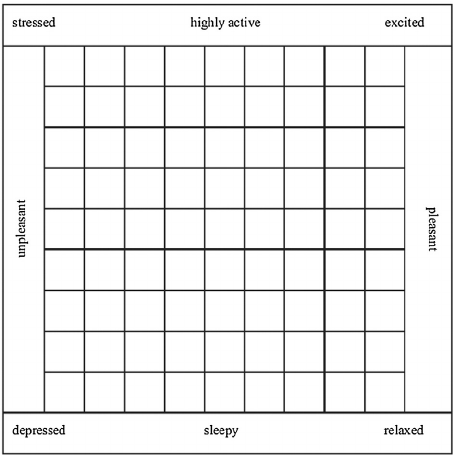
\includegraphics[width=0.6\textwidth]{affectgridbase.png}
\caption{Blank Affect Grid}
\label{fig:affectgrid}
\end{figure}

Ved anvendelse af dette grid kan en testperson nemt angive \textit{affect} ved at overveje deres nuværende fornøjelses- og ophidselsesniveau og derefter markere på gridet. Da dette ikke kræver meget af testpersonen, regner vi med at der kan markeres flere gange under evalueringen, uden at personen trækkes ud af interaktionen. Derfor anvender vi \textit{Affect Grid} til løbende at indsamle data om testpersonen \textit{affect} under evalueringen.

\section{3E}\label{sec:3E}
Foruden det kvantitative fra \textit{Affect Grid} ønsker vi også at indsamle kvalitativ data om testpersoners oplevelse. Mens kvantitativ data er let at opstille og sammenligne, kan kvalitativ data give en dybere forståelse af den enkelte testperson og deres oplevelse. For ikke at forstyrre testpersonen med endnu en metode under interaktionen, ønsker vi at bruge en metode der kan benyttes efterfølgende. Den skal altså kunne bruges på episode plan.

Vi vælger da at anvende metoden \textit{Expressing Experiences and Emotions} (\textit{3E}) udviklet af Marika Tähti og Marketta Niemelä\cite{3E}. Her får testpersonen udleveret et stykke papir, hvorpå der er tegnet en tændstikmand, en taleboble og en tænkeboble. Et eksempel kan ses på \cref{fig:3E}. De bliver da bedt op at tegne på papiret med henblik på at projektere deres oplevelser og følelser. Dette lader personen udtrykke sig på en nem og useriøs måde. Tændstikmandens formål er at opstille nogle rammer som personen kan udtrykke sig i. Dog må man tegne hvorend man vil på papiret. \textit{3E} er videreudviklet fra \textit{Emocards}. Her vælger en testperson fra et udvalg af tegneserieansigter, det ansigt der bedst repræsenterer, hvordan de føler\cite{EmoCard}. Med den blanke tændstikmand er det tanken, at testpersonen har større mulighed for at udtrykke sig end med førnævnte metode. 

\begin{figure}[h]
\centering
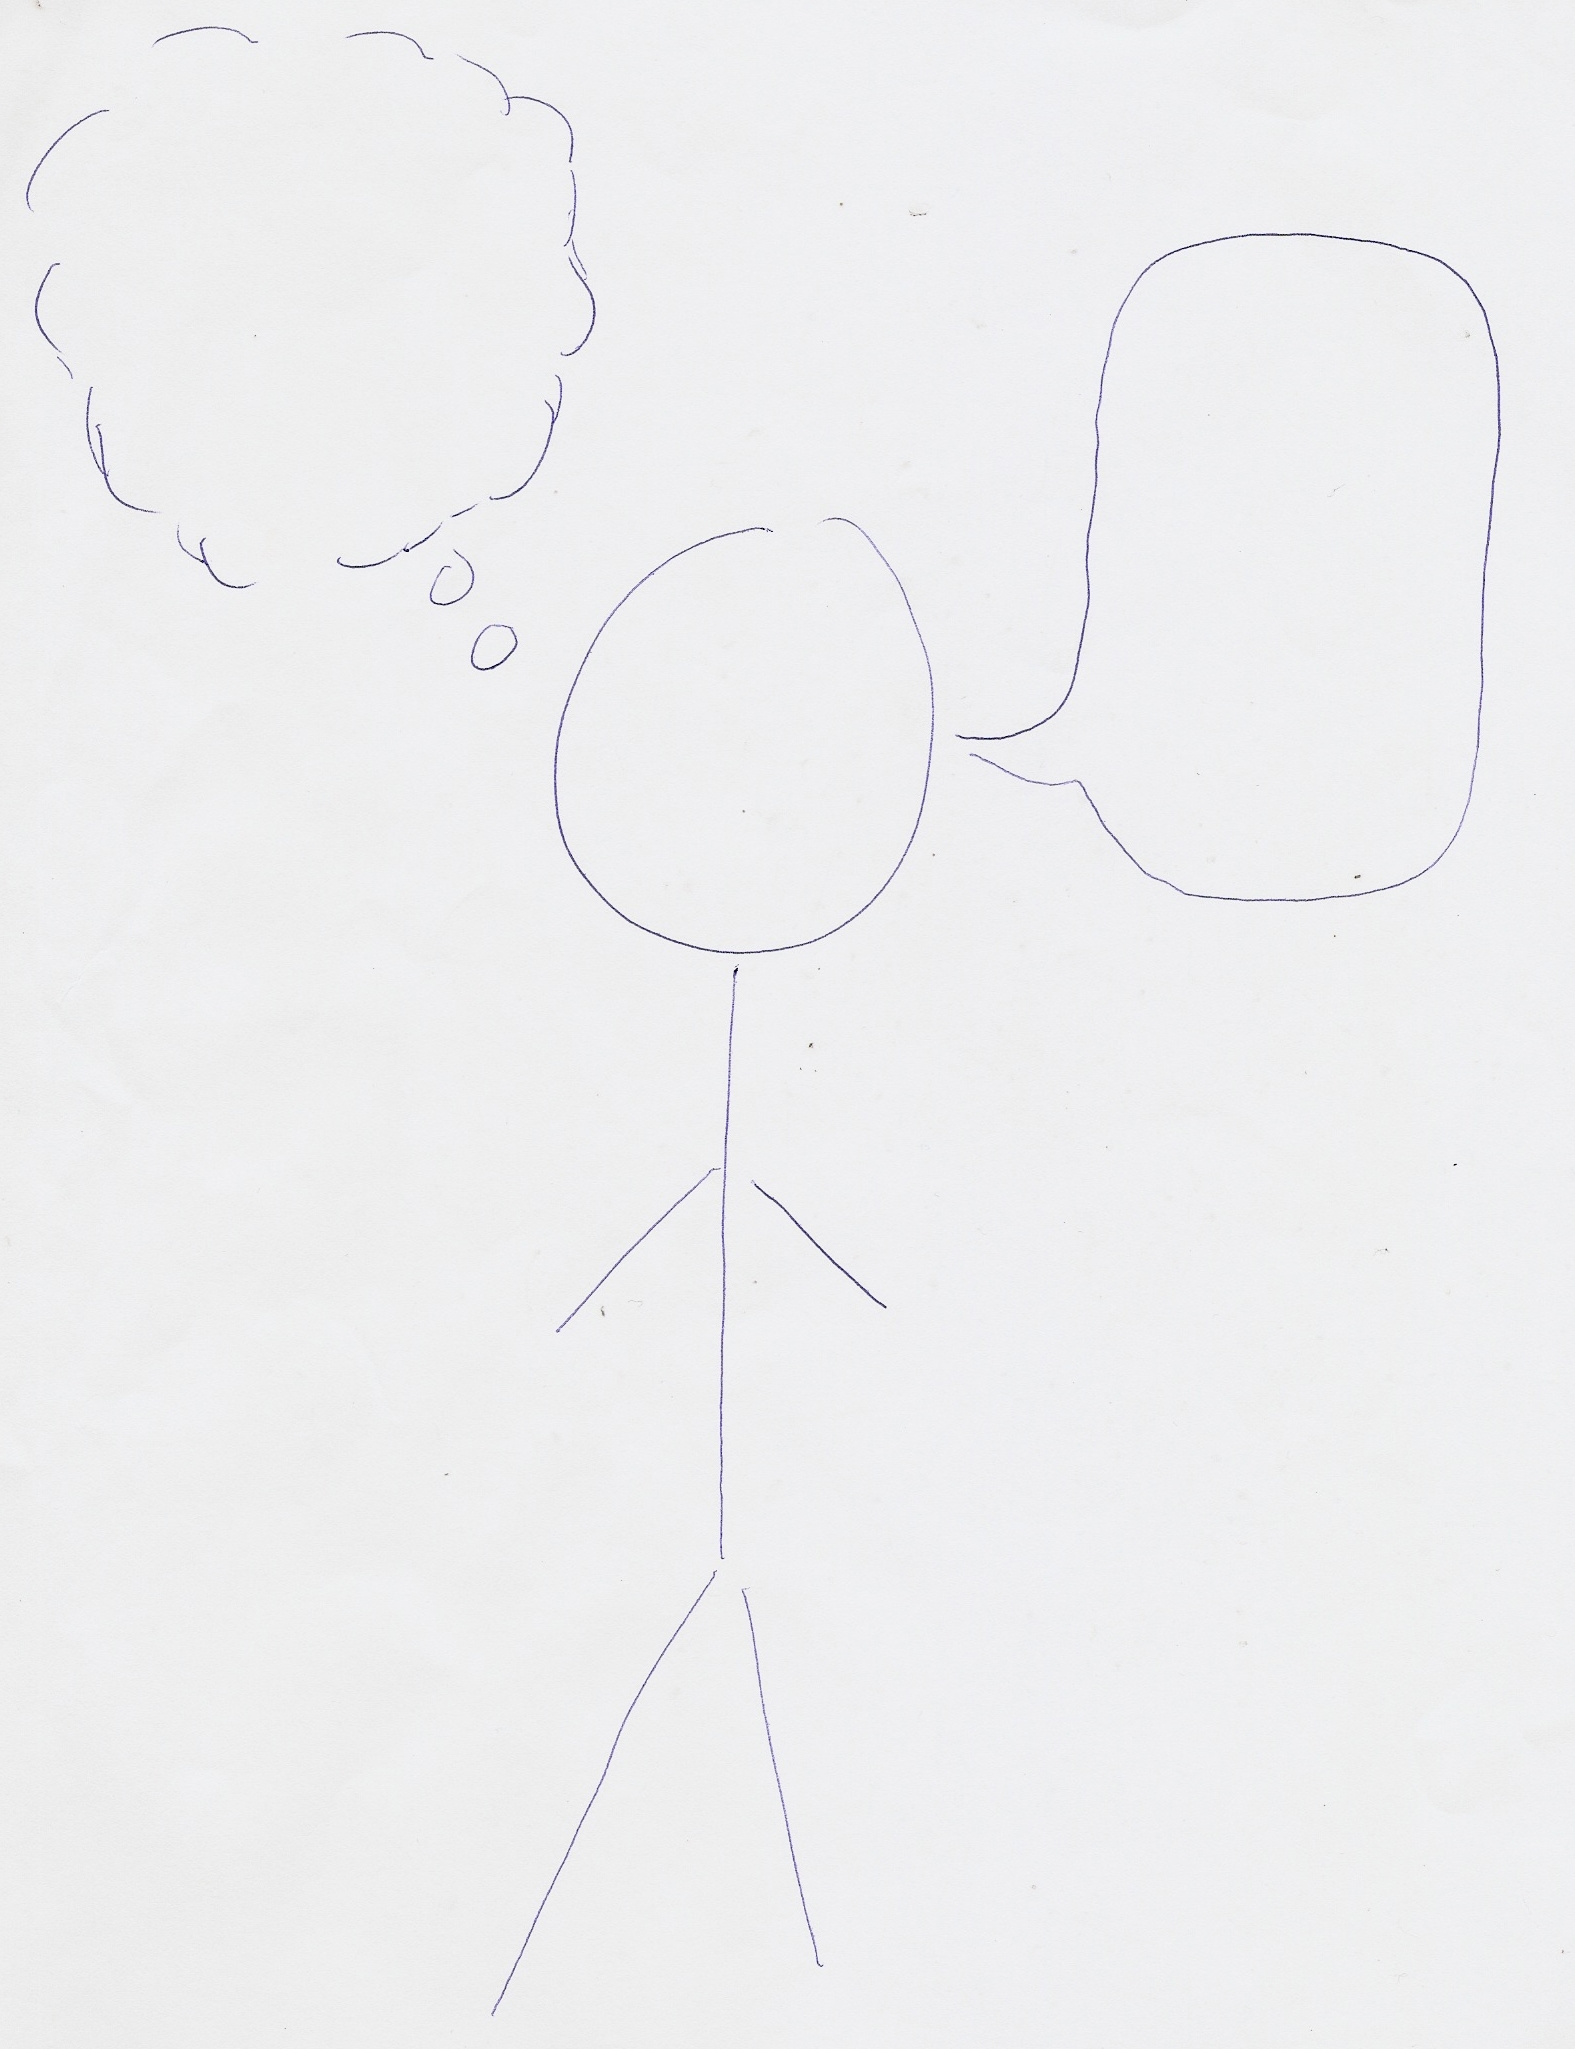
\includegraphics[width=0.6\textwidth]{3EBlank.jpg}
\caption{Blank 3E}
\label{fig:3E}
\end{figure}

Et problem med \textit{3E} er at det er svært at analysere dataene bagefter, da den kan fortolkes på mange måder. Derfor bedes testpersonen om at forklare deres tegning under eller efter udførsel.  